\documentclass[oneside,12pt]{amsart}
\usepackage[english]{babel}
\usepackage{graphicx}
\usepackage{float}
\usepackage{mathtools}
\usepackage{amsfonts}
\usepackage{amssymb}
\usepackage{siunitx}
\usepackage{amsthm}
\usepackage{enumitem}
\usepackage{stmaryrd}
\usepackage{multirow}
\usepackage[backend=bibtex,style=numeric]{biblatex}
\bibliography{Biblio}
\usepackage[a4paper, total={6in, 10in}]{geometry}
\graphicspath{{./}{}}% You can add the path for the images in the empty brackets 
\title{Capacitors: Wiring Parallel and in Series }
\author{Josh Goldfaden, Daniel Briseno}
\date{}
\newdimen\graph
\graph=4.2in
\newdimen\medgraph
\medgraph = 5.3in
\newdimen\smallgraph
\smallgraph = 3in
\newdimen\tinygraph
\tinygraph = 1.5in
\renewcommand{\arraystretch}{1.5}
\begin{document}
	\maketitle
	\section{Abstract}
	\indent In this lab, the effective capacitance of three virtual capacitors, labeled A, B, and C, was studied when these provided capacitors were both wired in series as well as parallel to one another. These observations were experimentally verified by arranging three green ceramic disc capacitors labeled “A,” “B,” and “C” in series as well as parallel to one another. Using a Digital Multi-meter, it was determined that the expected and actual capacitance (nF) of each arrangement had minimal discrepancies. In the second portion of this lab, a virtual capacitor constructed from two large, parallel conducting plates was studied. It is noteworthy that this virtual capacitor was the subject of a “movie” clip integrated with an interactive Logger Pro file. Particularly, the change in voltage spread across each plate was analyzed as the plates were moved further apart from one another. It was found that as the distance between the plates increased, the voltage reading proportionally increased. 
	\section{Introduction}
	\indent A capacitor is a system of any two conductors that are separated by an insulator. Each of the conductors in a capacitor carry net excess charge that are equal in magnitude but are opposing charges. The capacitance, the ability of a system to store charge which is mathematically denoted as C, can be expressed as the following: 
	\begin{align*}
		C = \frac{Q}{V}
	\end{align*}
	where $ Q $ is the magnitude of excess charge possessed by each conductor and $V$ is the potential difference (potential) across both conductors.\\
	
	\indent Gauss’ Law can be implemented to demonstrate that in an ideal parallel plate capacitor (a depiction of which is shown in Figure \ref{Ideal}), capacitance is directly related to the area $A$ of the plates. Further, Gauss’ Law displays that the capacitance of this ideal parallel plate system is inversely related to the distance $d$ between the two plates: 
	\begin{align*}
		C = \frac{\kappa \epsilon _{0}A}{d}
	\end{align*}
	where  $\kappa$ is the dielectric constant that is dependent upon the properties of the insulator between the two conductive plates, and $\epsilon_0$ is the electric constant, often referred to as ''permittivity".\\
	\begin{figure}[H]
		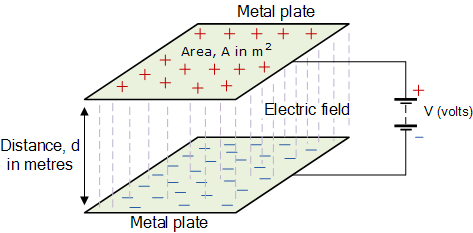
\includegraphics[width=\smallgraph,scale=0.01]{IdealCapacitor.png}
		%h (here) - same location
		%t (top) - top of page
		%b (bottom) - bottom of page
		%p (page) - on an extra page5
		%! (override) - will force the specified location
		\caption{Ideal plate capacitor}
		\label{Ideal}
	\end{figure}

	\indent We often connect capacitors to each other in series and in parallel. A depiction of capacitors in parallel can be seen in Figure \ref{Parallel}.\\
	 
	\begin{figure}[h]
		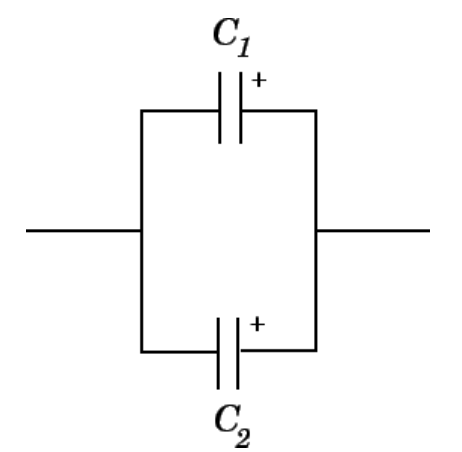
\includegraphics[width=\smallgraph,scale=0.01]{Parallel.png}
		%h (here) - same location
		%t (top) - top of page
		%b (bottom) - bottom of page
		%p (page) - on an extra page5
		%! (override) - will force the specified location
		\caption{Capacitors in parallel. Photo credit \cite{cap}}
		\label{Parallel}
	\end{figure}
\begin{figure}[h]
	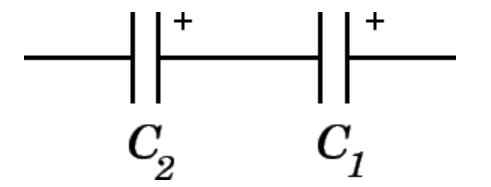
\includegraphics[width=\smallgraph,scale=0.01]{Series.png}
	%h (here) - same location
	%t (top) - top of page
	%b (bottom) - bottom of page
	%p (page) - on an extra page5
	%! (override) - will force the specified location
	\caption{Capacitors in series. Photo credit \cite{cap}}
	\label{Series}
\end{figure}

	\indent In this case we know that the voltage across the two capacitors is equal\cite{cap} and thus we can derive :
	\begin{align*}
	C_{total} &= \frac{Q_{total}}{V} \\
	&=\frac{Q_1+Q_2}{V}\\
	&= \frac{Q_1}{V} + \frac{Q_2}{V}\\
	&= C_1 + C_2
	\end{align*}
	
	\indent Figure \ref{Series} shows two capacitors connected in series. In this case we know that the excess charge $Q$ across both capacitors must be equal \cite{cap}, and we similarly compute:\\
	\begin{align*}
		\frac{1}{C_{total}} &= \frac{V}{Q}\\
		&= \frac{V_1 + V_2}{Q}\\
		&= \frac{V_1}{Q} + \frac{V_2}{Q}\\
		&= \frac{1}{C_1} + \frac{1}{C_2}
	\end{align*}


	\indent In summary, we can have the following four relations:
	\begin{align}
	&\text{Definition of capacitance} &&	C = \frac{Q}{V}\\
	&\text{For an ideal capacitor} &&C = \frac{\kappa \epsilon _{0}A}{d}\\
	&\text{For capacitors in paralel} &&C_{total} = C_1 + C_2\\
	&\text{For capacitors in series} && \frac{1}{C_{total}} = \frac{1}{C_1}+\frac{1}{C_2}
	\end{align}
	
	\section{Experimental confirmation of equations 2 and 3}
	\indent In this section of the experiment we seek to gain empirical confirmation of equations (2) and (3) derived in the introduction.\\
	
	\indent In order to do this, we measured the capacitance of three capacitors A,B, and C. The results of these measurements can be seen in Table \ref{abc} 

	\begin{table}[H]
		\begin{tabular}{ |c|c|}
			\hline
			Capacitor & Measured Capacitance (nF)\\
			\hline
			A&105.8\\
			B&99.9\\
			C&121.1\\
			\hline
		\end{tabular}
		\caption{Capacitance of capacitors A,B, and C.}
		\label{abc}
	\end{table}

	\indent After taking these measurements, we used equation (3) predicted the capacitance of all parallel circuits we could make using the three capacitors, then we built the circuits and measured the actual capacitance. This process was repeated for circuits in series with equation (4), and the results are seen in Tables \ref{inParallel} and \ref{inSeries}, respectively. 
	\begin{table}[H]
		\begin{tabular}{ |c|c|c|c|}
			\hline
			Capacitors & Theoretical Capacitance(nF)& Measured Capacitance(nF) &\% Error\\
			\hline
			A and B	&205.7&205&0.341\\
			A and C&226.9 & 226&0.398\\
			B and C&221&220&0.455\\
			A, B and C&326.8&327&0.0612\\
			\hline
		\end{tabular}
		\caption{Capacitance of A,B, and C connected in parallel.}
		\label{inParallel}
	\end{table}

\begin{table}[H]
	\begin{tabular}{ |c|c|c|c|}
		\hline
		Capacitor & Theoretical Capacitance(nF)& Measured Capacitance(nF) &\% Error\\
		\hline
		A and B&51.4&51.2&0.391\\
		A and C&56.5&56.5&0\\
		B and C&54.7&54.4&0.552\\
		A, B and C&36.1&35.9&0.557\\
		\hline
	\end{tabular}
	\caption{Capacitance of A,B, and C connected in series.}
	\label{inSeries}
\end{table}
	
	As expected, our predictions are very close to our measured values, with a maximum error of 0.455\% for the parallel condition, and 0.557\% for the series condition. With such small errors, we can clearly say that we have strong evidence in favor of equations (3) and (4) and that our small errors are likely due to measurement inaccuracies. 
	\newpage
	
\printbibliography
	 
	
\end{document}